\label{sec:breakout}
Here the agent needs to master the atari game breakout, see \autoref{fig:breakout}. The agent controls a small bar at the bottem of the screen with possible actions: move left, move right or stay. A ball moves with constant speed through the envirement. If the agent positions the small bar such that the ball hits the bar the ball inverts its vertical velocity bouncing upwards. Whenever the ball hits the bottem of the screen it disappears, the agent loses a life (it starts with 5) and a new ball is introduced with a random direction downwards. When the ball hits the left and right side of the screen the horizontal velocity is inverted making it bounce of the walls. Somewhat below the top of the screen is a stack of rows of blocks. Whenever the ball hits one of the blocks: the block disappears, the ball inverts its vertical velocity and the agent is rewarded with score one for the current timestep. If the ball hits the top of the screen its vertical velocity is inverted, bouncing it off the top. 

\begin{marginfigure}
    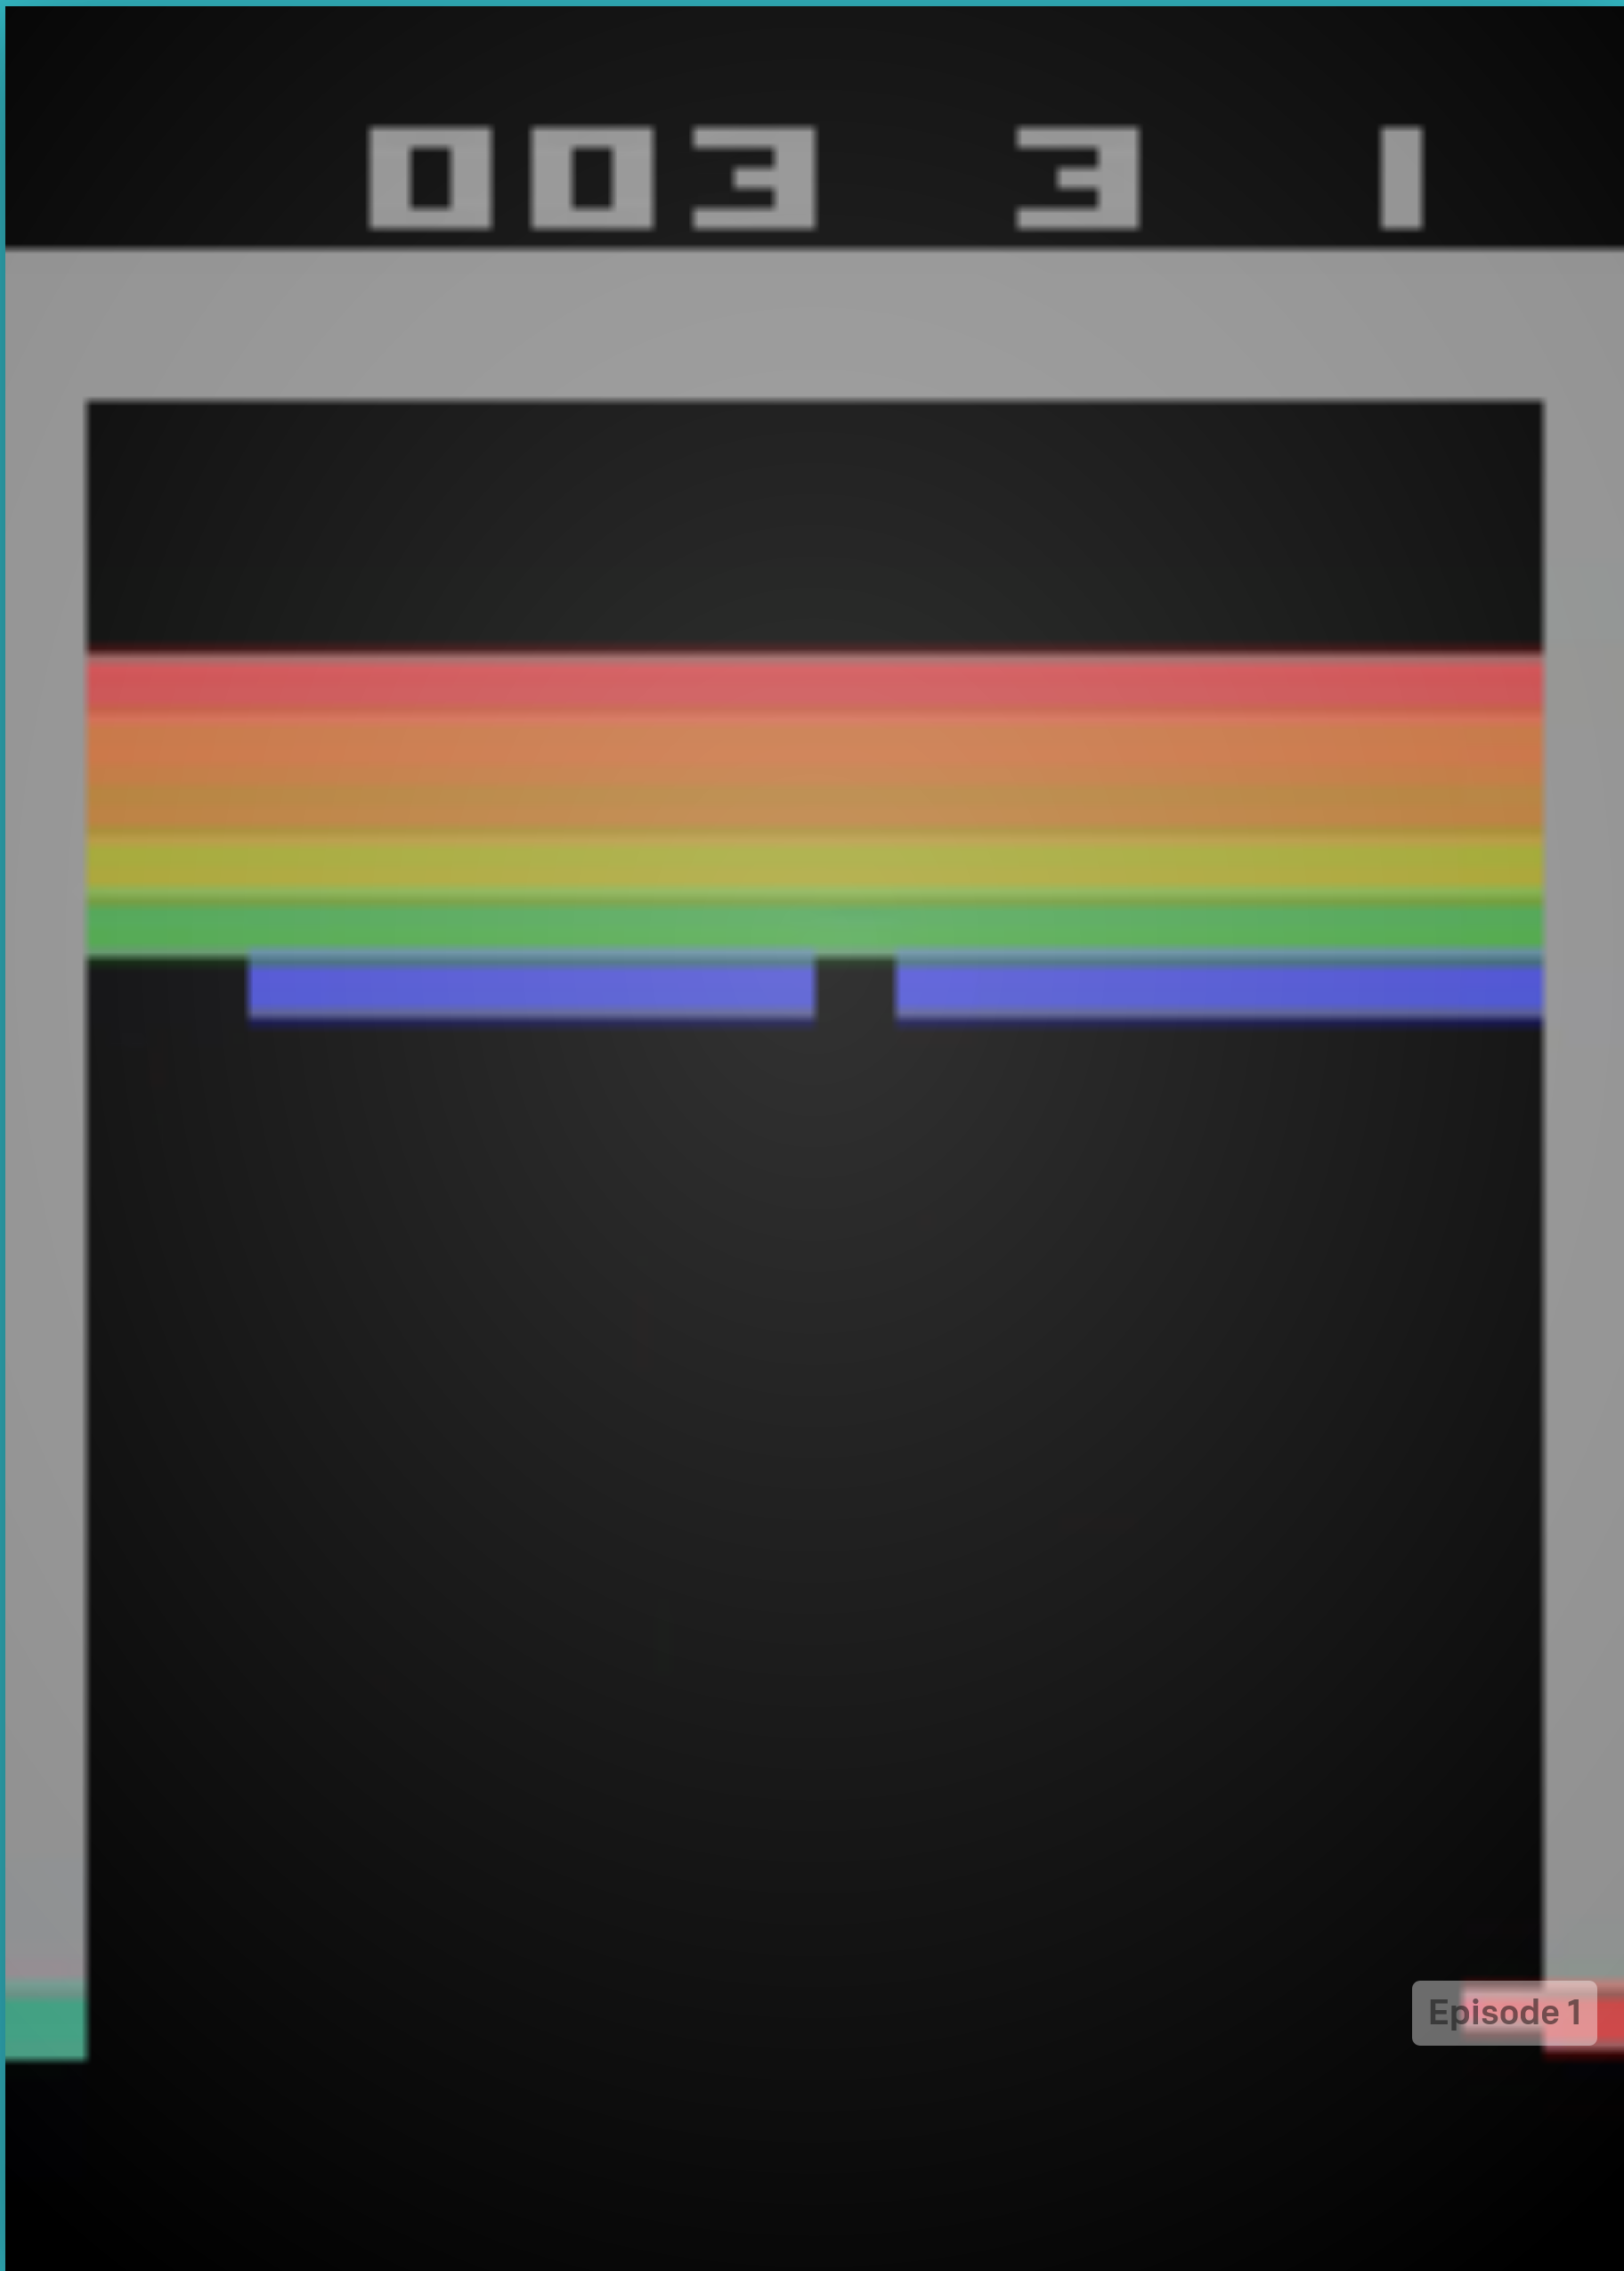
\includegraphics{breakout}
    \caption{The atari breakout envirement}
    \label{fig:breakout}
\end{marginfigure}

In this problem agent gets the same information as a human would, the pixels on the screen. Aditionally we give it the reward of the current timestep. Due to the computational complexity we do not want the agent to process the whole screen each timestep. We build our implementation on top of the \texttt{BreakoutDeterministic-v4} envirement provided by the \textit{openAI gym} project. This envirement returns the game state only once every 4 frames lowering the computational requirements.

\subsection{Implementation}
Initially we used a slightly adapted version of the mountain car DQN implementation described in \autoref{sec:mcar_impl}. The simple multilayer dense neural network was replaced with a convolutional neural network consisting of 2 layers both with kernal size 3 followed by two dense layers. The frames from the envirment where changed to greyscale and cropped to $80$ by $72$ pixels. This leaves the game envirement intact but removes the score at the top and ornamental edges, leaving an images as in \autoref{fig:breakout_postprocess} for the network.

This did not result in any learning by the agent. I tried multiple different networks before taking a look at related literature\cite{atari}. This lead to the conclusion that my agent was that my hyper paramaters where far from where they should be.

Taking the hyperparamaters from the famouse "Human-level control through deep reinforcement learning"\cite{DQN} we start changing the implementation. The mountain car agent is limited in the number of training sessions, this does not make sense for the breakout agent as we want to limit the number of steps not training sessions. From the perspective of a human traning there is no difference between losing a life and the game restarting however the agent was not even punished for losing a life. That was changed so losing a life is treated as losing the game during training.
Using only one frame as input to the network does not allow the agent to use the concept of direction or speed, essential to a human player. As in\cite{DQN} we feed the network a stack of the last 4 frames, as given to us by the envirement, for prediction and during training. 

\begin{marginfigure}
    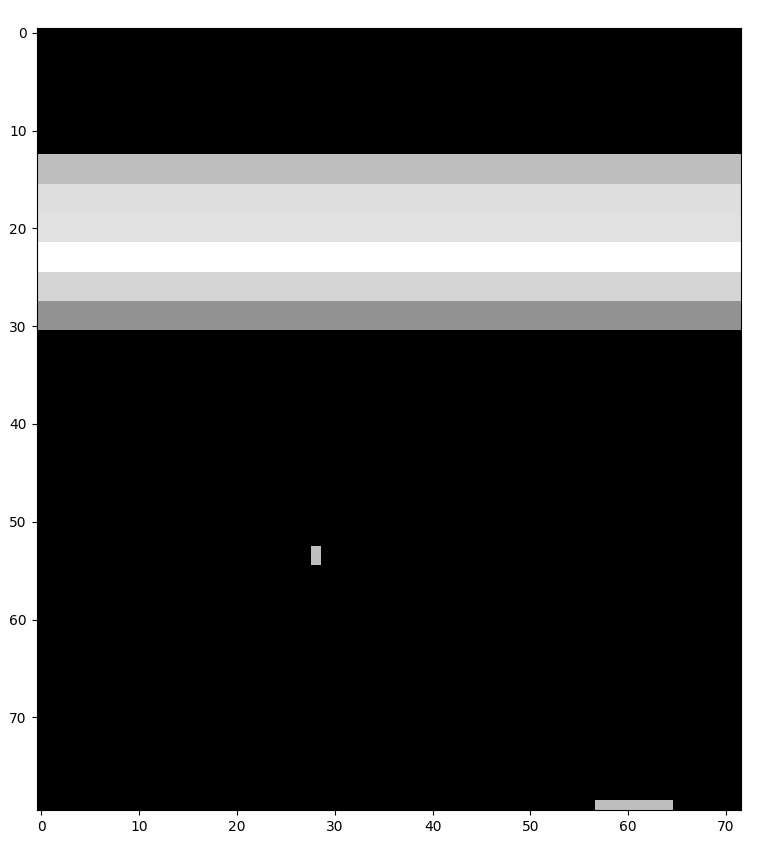
\includegraphics{network_input}
    \caption{A frame returned by the atari breakout envirement after postprocessing for our agent, converting to color and cropping out the unneeded edges}
    \label{fig:breakout_postprocess}
\end{marginfigure}

These changes give a number of implementation problems. We can not take any action for the first 3 timesteps as we can not make a stack of 4 frames to feed the agent. We have removed the training in sessions however we should not use frames from another training session. For example is the games has ended in frame $x$ we can not use the network until frame $x+4$. To enforce this we use the function \texttt{reset}. It resets the envirement and forwards the game 3 timesteps without taking any action. We use a new class \texttt{State} to keep track of the 4 frames. I provides a method \texttt{push} that takes as arguments an before and after state together with the action taken, score and if the game is over. It then forgets the oldest before and after state adding the new state to its internal stack.